\section*{Results}
\label{sec:results}

We evaluated representation-pairing kernels for set-intersection cardinality. Throughout, we use
\emph{cell} to denote one representation pairing (for example $\cell{\rB}{\rS}$), \emph{variant} to
denote one implementation of a cell, and \emph{pairing matrix} to denote the full set of cells;
unless stated otherwise, every ratio is reported against a \texttt{run\_optimize}-tuned CRoaring
baseline. Figure~\ref{fig:pairing-matrix} lays out that matrix: the five representation families,
the driving variable each pairing's cost is proportional to, and the path from precomputed row
metadata through the selector to a chosen kernel.

The mechanisms reported here form a progression ordered by what a caller gives up, not by what each
costs. Choosing a representation (Fig.~\ref{fig:pairing-matrix}a--b) and consulting a zone map
(Fig.~\ref{fig:density-sweep}a) give up nothing: the question and the answer are unchanged, and
only the work changes. Prefix filtering and a size bound narrow the question instead --- only pairs
above a similarity threshold, or within a size band --- and are available only because the caller
said what they wanted; they are opt-in, never substituted for the first two, and their return is
analytic rather than measured here, reaching as little as a few per cent of pairs surviving at a
high similarity threshold (Methods, ``What makes work avoidable''; see Supplementary Note~\ref{note:threshold} and
Supplementary Fig.~\ref{fig:prefix} for the derivation and the composition rule that governs when
the two may be multiplied together). Batch amortisation leaves the contract unchanged again but
needs many operations rather than one, because what it removes is repetition rather than work.

\begin{figure}[!t]
\centering
% ===========================================================================
% Figure 1 — overview. Body only; \input inside a figure environment.
% House idiom follows the scaffold paper's fig:planes: minipage panels with
% bold letter labels, \resizebox per panel, and the two-saturation convention
% (strong fill = the lanes the panel is about, faint same-hue fill = context).
%
% Requires simdgrid.sty and the repr* colours from storm.tex.
% ===========================================================================

% Focus / context saturations, one pair per representation.
\colorlet{focB}{reprB!45}\colorlet{ctxB}{reprB!12}
\colorlet{focS}{reprS!55}\colorlet{ctxS}{reprS!14}
\colorlet{focR}{reprR!55}\colorlet{ctxR}{reprR!14}
\colorlet{focW}{reprW!55}\colorlet{ctxW}{reprW!14}
\colorlet{focC}{reprC!65}\colorlet{ctxC}{reprC!18}
\colorlet{zone}{black!18}

\tikzset{
  gridcell/.style={draw=black!55, line width=0.4pt, minimum width=16.5mm,
                   minimum height=6.6mm, inner sep=1pt, font=\scriptsize,
                   anchor=center},
  hdr/.style={font=\scriptsize\bfseries},
  flowbox/.style={draw=black!60, rounded corners=1.2pt, align=left,
                  font=\scriptsize, inner sep=3.2pt},
  flowarrow/.style={-{Latex[length=1.8mm]}, draw=black!65, line width=0.5pt},
}

% Type size. Both panels are \resizebox'd to their minipage, so the size a
% label renders at is (its point size) x (panel width / panel natural width),
% and nothing else. Measured naturals: panel a 243.8 pt at \simdcw 4.6mm,
% panel b 230.2 pt. At the previous .50/.435 split with \tiny cells, panel a's
% digits rendered 5.1 pt against panel b's 7.6 pt -- and against panel a's OWN
% 8.2 pt row labels and position ruler, which are \scriptsize.
%
% Fixed by making every glyph in panel a one size (\scriptsize, as its labels
% already were) and widening the cell so the longest token, the run record
% 12:3, still fits inside it -- cells must stay a uniform width or the strips
% stop comparing item counts, which is the panel's whole point. The two
% minipage widths are then set so both panels land at ~7 pt, matching the
% 8 pt body size of the matplotlib panels elsewhere in the paper.
\begin{minipage}[b]{.54\linewidth}
\setlength{\simdcw}{6.0mm}% local to this minipage; fits "12:3" at \scriptsize
\textbf{a}\par\vspace{0.6mm}
\resizebox{\linewidth}{!}{%
\begin{simdpicture}
  \simdstrip[font=\scriptsize\ttfamily]{5.4}{\rB}{%
    0/ctxB,1/focB,1/focB,1/focB, 0/ctxB,0/ctxB,0/ctxB,0/ctxB,%
    0/ctxB,0/ctxB,0/ctxB,0/ctxB, 1/focB,1/focB,1/focB,0/ctxB}
  \simdlabels{4.85}{0}{15}
  \node[simd note, anchor=east] at (-0.35,4.85) {position};
  \simdstrip[font=\scriptsize\ttfamily]{3.1}{\rS}{%
    1/focS,2/focS,3/focS,12/focS,13/focS,14/focS}
  \simdstrip[font=\scriptsize\ttfamily]{1.55}{\rR}{{1{:}3}/focR,{12{:}3}/focR}
  \simdstrip[font=\scriptsize\ttfamily]{0}{\rW}{L/focW,{F0}/ctxW,L/focW}
\end{simdpicture}}
\end{minipage}\hfill
% ------------------------------------------------------------------ panel b
\begin{minipage}[b]{.395\linewidth}
\textbf{b}\par\vspace{0.6mm}
\resizebox{\linewidth}{!}{%
\begin{tikzpicture}[x=1mm,y=1mm]
  % Row labels sit to the RIGHT of the grid, level with their cells, matching
  % the pair matrix in panel d.
  \foreach \c/\i in {\rB/0,\rS/1,\rR/2,\rW/3}{
    \node[hdr] at (\i*17.5,5.2) {\c};
    \node[hdr, anchor=west] at (61.8,-\i*7.1) {\c};
  }
  \node[gridcell, fill=focB]  at (0,0)      {$\Theta(m)$};
  \node[gridcell, fill=ctxS]  at (17.5,0)   {$\Theta(|S|)$};
  \node[gridcell, fill=ctxR]  at (35,0)     {$\Theta(r)$};
  \node[gridcell, fill=ctxW]  at (52.5,0)   {$\Theta(\ell{+}g)$};
  \node[gridcell, fill=ctxS]  at (17.5,-7.1){$\Theta(|A|{+}|B|)$};
  \node[gridcell, fill=ctxR]  at (35,-7.1)  {$\Theta(|S|{+}r)$};
  \node[gridcell, fill=ctxW]  at (52.5,-7.1){$\Theta(|S|{+}\ell{+}g)$};
  \node[gridcell, fill=ctxR]  at (35,-14.2) {$\Theta(r_A{+}r_B)$};
  \node[gridcell, fill=ctxW]  at (52.5,-14.2){$\Theta(r{+}\ell{+}g)$};
  \node[gridcell, fill=ctxW]  at (52.5,-21.3){$\Theta(\ell{+}g)$};
  % Lower triangle: drawn but empty. The matrix is symmetric, so these cells
  % carry no information and saying so in every one of them is noise.
  \foreach \x/\y in {0/-7.1, 0/-14.2, 17.5/-14.2, 0/-21.3, 17.5/-21.3, 35/-21.3}{
    \node[gridcell, fill=black!3, draw=black!25] at (\x,\y) {};
  }

  % The complement, shown rather than described: a dense side becomes a sparse
  % one, and re-enters the same ten cells.
  \begin{scope}[shift={(-8,-31)}]
    \foreach \bit [count=\k from 0] in {1,1,1,0,1,1,1,1,1,0,1,1,1,1,0,1}{
      \ifnum\bit=1 \def\f{focB}\else\def\f{white}\fi
      \draw[draw=black!55, line width=0.35pt, fill=\f]
        (\k*4,0) rectangle ++(4,4.4);}
    \node[hdr, anchor=east] at (-1.5,2.2) {$A$};
    \foreach \bit [count=\k from 0] in {0,0,0,1,0,0,0,0,0,1,0,0,0,0,1,0}{
      \ifnum\bit=1 \def\f{focC}\else\def\f{white}\fi
      \draw[draw=black!55, line width=0.35pt, fill=\f]
        (\k*4,-8) rectangle ++(4,4.4);}
    \node[hdr, anchor=east] at (-1.5,-5.8) {$A^{c}$};
    \draw[flowarrow] (68,2.2) -- ++(5,0) |- (68.01,-5.8);
  \end{scope}
\end{tikzpicture}}
\end{minipage}

\caption{\textbf{The object of study: equivalent encodings of one set, and the matrix of kernels
that pairing them gives.}
\textbf{a}, One set of six elements over a 16-position universe, encoded four ways. One cell is one
stored item, so a strip's length is the number of items that encoding must touch: 16 bits for $\rB$
($\Theta(m)$, whatever the set holds), six values for $\rS$ ($\Theta(|X|)$), two
$(\mathit{start}{:}\mathit{length})$ records for $\rR$ ($\Theta(r)$, whatever the runs' lengths), and
three words --- two literal and one fill --- for $\rW$ ($\Theta(\ell+g)$). Note that a cell is a bit
in $\rB$ and a word in the others, so the strips compare work, not bytes. Strong fill marks set
positions, and the position ruler applies to $\rB$ alone, the only positional encoding.
\textbf{b}, Pairing two representations gives a kernel with its own cost function. The matrix is
symmetric, so ten cells are distinct, and \emph{only} $\cell{\rB}{\rB}$ is linear in the universe
$m$; every other cell is sub-linear in it. Above density one half a side is handled through its
complement ($\rC$), shown beneath: a dense operand becomes a sparse one and re-enters the same ten
cells, with the answer recovered by inclusion--exclusion. Costs are derived in Methods.
Schematic; no measured data.}
\label{fig:pairing-matrix}
\end{figure}

\subsection*{The cost of intersection is U-shaped in density}
\label{sec:r1}

We separate the cost of intersection along density -- more precisely, each row's distance from
density one half. To determine whether the fixed cost assumed of bitmap--bitmap intersection actually holds
across the range it is assumed to hold across, and where the remaining cells beat it, we swept
density from a single set bit to a fully set universe and measured every one of
\nm{count of pairing cells swept in the density sweep} cells at each point. Both sides were swept at
matched density with the universe pinned at \nm{universe size held fixed across the density sweep,
in bits} bits, so that cache residency -- \nm{cache level the density sweep is resident in, e.g.\
L2} throughout -- stayed constant along the axis instead of confounding it. The sweep in
Fig.~\ref{fig:density-sweep} covers the uniform spectrum; the $1/i$ spectrum, exercised identically,
is reported in Supplementary Fig.~\nm{number of the supplementary figure carrying the 1/i density
sweep}.

Bitmap--bitmap cost was flat across the swept range -- \nm{$\cell{\rB}{\rB}$ cost, ns per pair, range
across the density sweep} at the cache residency stated above, spanning
\nm{order-of-magnitude span of the density sweep} orders of magnitude of density -- which turns the
fixed-cost premise underlying the standard approach from an argument into a measurement. Against
that flat line, the best cell at the sparsest density point beat $\cell{\rB}{\rB}$ by
\nm{best-cell speedup over $\cell{\rB}{\rB}$ at the sparsest density point}, and the advantage grew
with universe size.

The two curves crossed at approximately \nm{crossover density, order of magnitude, stated as an
approximate value} -- an approximate value, since the exact crossover moves under re-measurement even
though its existence does not. Near density one, the curve turned again: a row that is almost
entirely set has a complement that is almost entirely empty, and \spec{we expect a complement-based
cell, $\cell{\rC}{\rB}$ or $\cell{\rC}{\rC}$, to win the dense tail as a designed strategy, beating the
margin achieved when $\cell{\rR}{\rR}$ wins only incidentally}, beating $\cell{\rB}{\rB}$
by \nm{dense-tail win ratio over $\cell{\rB}{\rB}$ at the densest measured point}. The result is a U,
not a monotonic curve, and it corrects the framing this project began with: the operative variable is
not sparsity but distance from density one half, since a row that is 99.99\% set is exactly as
compressible as one that is 0.01\% set (Fig.~\ref{fig:density-sweep}).

\begin{figure}[!p]
\centering
\footnotesize
\textbf{a}\par\vspace{0.4mm}
% Zone-map schematic (was Fig. 1c)
% Extracted from the former Fig. 1; rendered as a panel of its own figure.
\centering
% ===========================================================================
% Figure 1 — overview. Body only; \input inside a figure environment.
% House idiom follows the scaffold paper's fig:planes: minipage panels with
% bold letter labels, \resizebox per panel, and the two-saturation convention
% (strong fill = the lanes the panel is about, faint same-hue fill = context).
%
% Requires simdgrid.sty and the repr* colours from storm.tex.
% ===========================================================================

% Focus / context saturations, one pair per representation.
\colorlet{focB}{reprB!45}\colorlet{ctxB}{reprB!12}
\colorlet{focS}{reprS!55}\colorlet{ctxS}{reprS!14}
\colorlet{focR}{reprR!55}\colorlet{ctxR}{reprR!14}
\colorlet{focW}{reprW!55}\colorlet{ctxW}{reprW!14}
\colorlet{focC}{reprC!65}\colorlet{ctxC}{reprC!18}
\colorlet{zone}{black!18}

\tikzset{
  gridcell/.style={draw=black!55, line width=0.4pt, minimum width=16.5mm,
                   minimum height=6.6mm, inner sep=1pt, font=\scriptsize,
                   anchor=center},
  hdr/.style={font=\scriptsize\bfseries},
  flowbox/.style={draw=black!60, rounded corners=1.2pt, align=left,
                  font=\scriptsize, inner sep=3.2pt},
  flowarrow/.style={-{Latex[length=1.8mm]}, draw=black!65, line width=0.5pt},
}

% ------------------------------------------------------------------ panel c
\resizebox{.506\linewidth}{!}{%
\begin{simdpicture}
  % One verdict per bin, carried as a colour down the whole column, so the
  % reader can trace a bin top-to-bottom. Colour here is the SAME reserved
  % cost/saving axis used in the matplotlib panels of this figure and of
  % Supplementary Fig. S1, and it means the same thing in all of them:
  %   workc  = there is data here, so this bin costs work
  %   avoidc = nothing here, so the work is skipped
  % It formerly ran green-for-occupied against red-for-empty, which inverted
  % the sense of green between this panel and panel e (where green marked work
  % NEVER done) and spent R's representation hue on a non-representation
  % meaning. Neither is true now.
  %
  % Colour is never the only encoding: the 0/1 digits, the tick/cross glyphs,
  % the fill/text-contrast pairing (white on the dark accent, black on the
  % light one) and the dashed bin rules each carry the verdict on their own,
  % so the panel reads in greyscale.
  \definecolor{workc}{HTML}{EE6677}
  \definecolor{avoidc}{HTML}{66CCEE}
  \colorlet{visitc}{workc}
  \colorlet{skipc}{avoidc}

  % Each row is coloured by ITS OWN occupancy, so the AND row reads as the
  % product of the two above it: work AND work = work, work AND skip = skip.
  % Bin 1 is the instructive case -- B occupies it, A does not, so occ_B is
  % red, occ_A is cyan, and the pair skips the bin.
  %
  % Type size: cells were \tiny against \scriptsize row labels inside one
  % picture, so the digits rendered about 3.6 pt on the page. Both are
  % \scriptsize now and the picture is scaled to render at roughly 8 pt, the
  % same body size as the matplotlib panels beneath it.
  \foreach \bin/\ca/\ta/\cb/\tb/\cn/\tn/\abits/\bbits/\oa/\ob/\an in {%
      0/workc/white/workc/white/workc/white/{0,1,0,0}/{0,0,1,0}/1/1/1,
      1/avoidc/black/workc/white/avoidc/black/{0,0,0,0}/{0,0,1,0}/0/1/0,
      2/avoidc/black/avoidc/black/avoidc/black/{0,0,0,0}/{0,0,0,0}/0/0/0,
      3/workc/white/workc/white/workc/white/{0,1,0,0}/{0,0,1,0}/1/1/1}{%
    % Operand rows: light tint of that row's own verdict, set bits at full.
    % Text colour tracks the fill so every digit stays legible on both accents
    % -- white on the mid-tone red, black on the light cyan.
    \foreach \bit [count=\k from 0] in \abits {%
      \ifnum\bit=1\relax
        \node[simd cell, fill=\ca, text=\ta, font=\scriptsize\ttfamily]
          at (\bin*4+\k,2) {1};
      \else \node[simd cell, fill=\ca!15, text=black!60, font=\scriptsize\ttfamily]
          at (\bin*4+\k,2) {0};\fi}
    \foreach \bit [count=\k from 0] in \bbits {%
      \ifnum\bit=1\relax
        \node[simd cell, fill=\cb, text=\tb, font=\scriptsize\ttfamily]
          at (\bin*4+\k,0) {1};
      \else \node[simd cell, fill=\cb!15, text=black!60, font=\scriptsize\ttfamily]
          at (\bin*4+\k,0) {0};\fi}
    % summary rows, each in its own row's colour; the AND row is the product
    \node[simd cell, fill=\ca, text=\ta, font=\scriptsize\ttfamily,
          minimum width=4\simdcw] at (\bin*4,-1.7) {\oa};
    \node[simd cell, fill=\cb, text=\tb, font=\scriptsize\ttfamily,
          minimum width=4\simdcw] at (\bin*4,-3.1) {\ob};
    % the AND itself -- this is the mechanism, kept as bits
    \node[simd cell, fill=\cn, text=\tn, font=\scriptsize\ttfamily,
          minimum width=4\simdcw, line width=0.8pt, draw=black!70]
      at (\bin*4,-4.5) {\an};
    % and its readout, as a glyph. Glyphs are drawn dark rather than in the
    % accent itself, so they stay the panel's most legible encoding.
    \node[simd cell, fill=\cn!12, minimum width=4\simdcw,
          draw=\cn, line width=0.7pt] at (\bin*4,-5.9) {};
    \ifnum\an=1\relax
      \draw[line width=1.1pt, draw=workc!65!black, line cap=round, line join=round]
        (\bin*4+1.62,-5.40) -- (\bin*4+1.86,-5.68) -- (\bin*4+2.40,-5.08);
    \else
      \draw[line width=1.1pt, draw=avoidc!55!black, line cap=round]
        (\bin*4+1.72,-5.68) -- (\bin*4+2.28,-5.12)
        (\bin*4+1.72,-5.12) -- (\bin*4+2.28,-5.68);
    \fi
  }

  \node[simd label] at (-0.35,2.5) {$A$};
  \node[simd label] at (-0.35,0.5) {$B$};
  \node[simd label] at (-0.35,-1.2) {$\mathrm{occ}_A$};
  \node[simd label] at (-0.35,-2.6) {$\mathrm{occ}_B$};
  \node[simd label] at (-0.35,-4.0) {$\mathrm{occ}_A \wedge \mathrm{occ}_B$};
  \node[simd label] at (-0.35,-5.4) {visit?};
  \foreach \b in {0,4,8,12,16}{
    \draw[black!45, dashed, line width=0.35pt] (\b,-6.1) -- (\b,3.35);}
  \simdbrace{0}{16}{-6.5}{popcount $=2$: visit bins 0 and 3, skip half the universe}
\end{simdpicture}}


\vspace{0.4mm}
\par\vspace{1.0mm}
% The canvas is generated at exactly \textwidth, so it is included at full
% width and never scaled: at the previous .75 it rendered its 8 pt body text
% at 4.5 pt and its annotations below 4 pt.
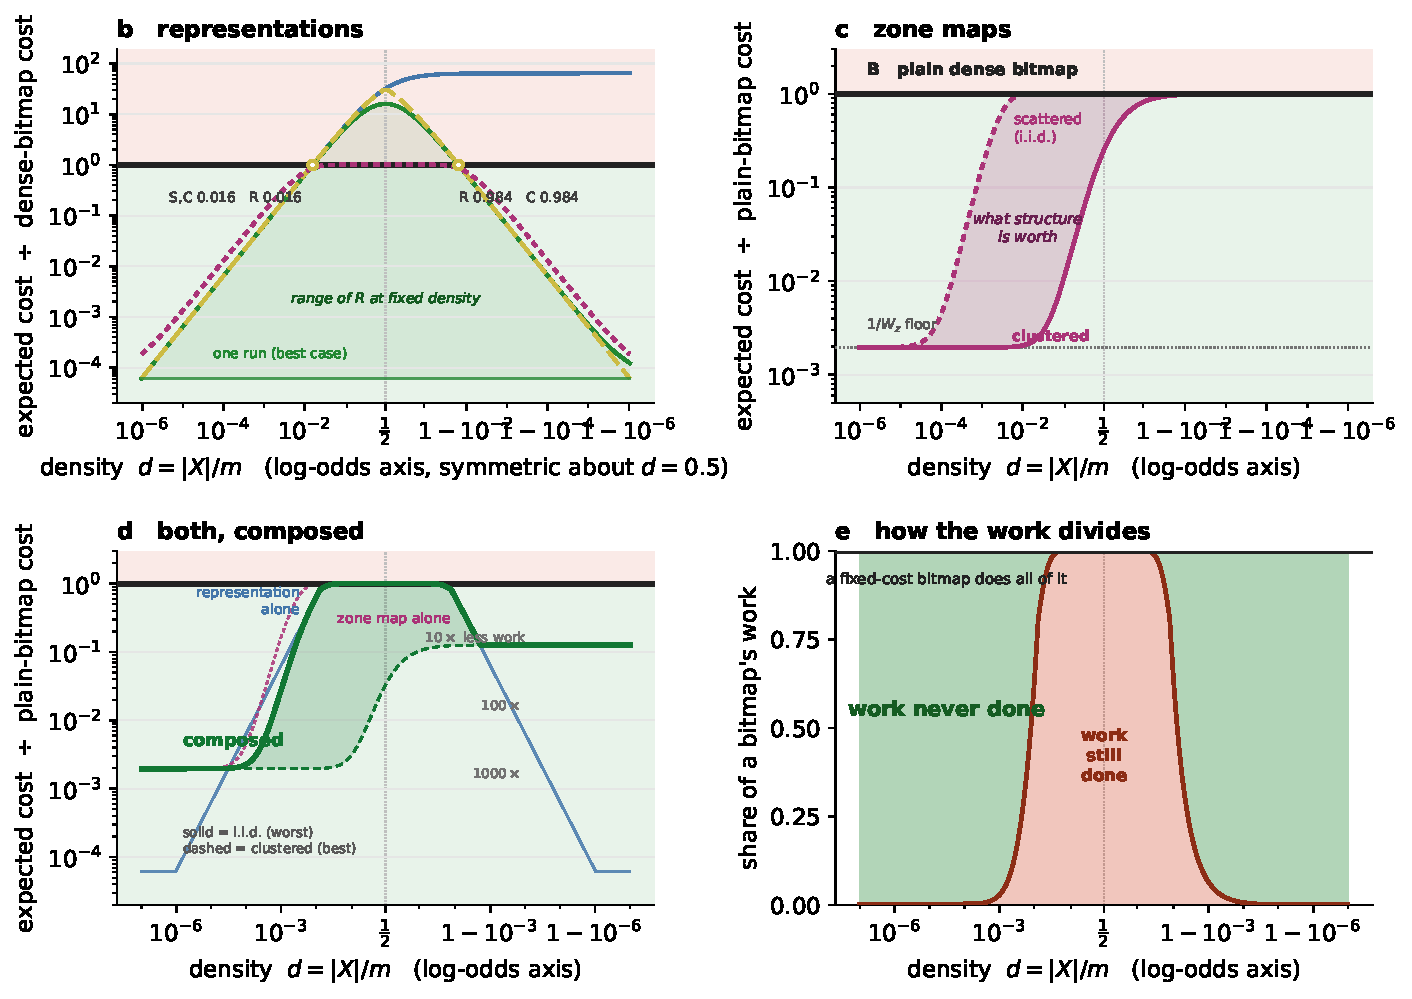
\includegraphics[width=\linewidth]{figures/fig2_expectations}
\caption{\textbf{What a fixed cost leaves on the table, analytically.} Derived, not measured; every
panel models \emph{work} rather than time. Reading key: hue names a representation, so mechanisms
are grey and separated by line style; red marks work still done, cyan work avoided, and grey shading
the region dearer than a plain bitmap.
\textbf{a}, A zone map within one pair. Each bin carries one bit recording whether that operand
holds anything in it, and $\mathrm{occ}_A \wedge \mathrm{occ}_B$ is the AND of the two summaries.
Follow bin~1: $B$ occupies it and $A$ does not, so the pair skips the bin even though one side holds
data there. The popcount of the AND is the \emph{exact} number of bins to visit, and a popcount of
zero proves the operands disjoint without reading either. Digits and glyphs repeat every verdict, so
the panel reads without colour.
\textbf{b}, Expected cost of each representation for a uniformly random set, as a multiple of the
dense-bitmap cost, on a log-odds density axis. Every cost is proportional to the universe $m$, so
this panel is scale-invariant and the crossovers are universal constants: open circles at
$d = 1/w = 0.0156$ for $\rS$ and $\rC$, $0.0159$ for $\rR$, and their complements. The bitmap is the
line at $1$. Shading marks the range of $\rR$ at fixed density --- one run at best, the i.i.d. value
at worst --- which is the deviation the method exploits.
\textbf{c}, The same for a zone map. Arrangement, not density, sets the share of bins an operand
occupies: at $d = 0.01$ and $W_z = 512$ the scattered and clustered extremes differ by
$482\times$, so the i.i.d. curve floors what a summary is worth.
\textbf{d}, The two composed. Filtering concentrates density, so the representation used inside a
surviving bin is the one for that bin's local density. Clustered, the composition costs $0.195\%$ of
a bitmap across the sparse range at $W_z = 512$, rising to $12.7\%$ only in the dense half; the knee
sits at $d = 1/8$ for every bin width.
\textbf{e}, The same as a division of labour: the share of a bitmap's work never done against the
share still done, taking the best of the four options at each density. $99.8\%$ is never done
at $d = 10^{-4}$; the waist about $d = \tfrac12$ is where a bitmap is the right kernel.
Measurements on real corpora appear on these axes in Supplementary Fig.~\nm{number}.}
\label{fig:density-sweep}
\end{figure}

Each mechanism above is a bet that the data deviates from randomness, and the size of the win at the
sparse extreme, the location of the crossover, and the two-sided condition under which a zone map is
worth consulting at all follow from a closed-form counting argument against the least favourable
(independent-placement) arrangement of elements, given in full in Supplementary Note~\ref{note:zonemap}. Inside the
band where nothing beats $\cell{\rB}{\rB}$ (Fig.~\ref{fig:density-sweep}d), no encoding is smaller
than the bitmap and no bin is empty, so the return there comes from throughput rather than
avoidance --- the axis the vectorized \texttt{AND}-and-popcount literature has already carried a
long way \cite{mula2018popcount}.

\subsection*{The winning representation pairing migrates across real corpora}
\label{sec:r2}

The sweep above varies density by construction, and a generator can always be
suspected of encoding exactly the structure its own kernels are built to exploit. We therefore
repeated the central comparison on corpora of independent provenance: the twelve corpora CRoaring's
own benchmark harness runs by default \cite{chambi2016roaring,lemire2018roaring}, together with
\prov{five} larger modern graphs, for \prov{17} corpora spanning \prov{$7.89\times10^{-7}$ to
$1.73\times10^{-1}$} in density and \prov{$1.995\times10^{5}$ to $3.697\times10^{7}$} bits in universe
size (full provenance, and the further corpora scored only against an all-bitmap baseline, in
Supplementary Table~\ref{tab:corpus-inventory}, Supplementary Note~\ref{note:corpora}). Every corpus is scored against
the same \texttt{run\_optimize()}-tuned CRoaring baseline used throughout Results, so this comparison
is continuous with the synthetic sweeps above rather than separate from them.

Table~\ref{tab:corpora} reports, for every corpus, universe size and density, the pairing cell that
won under best-cell (oracle) selection, and the ratio against tuned CRoaring and against an
all-bitmap baseline. Both ratios are oracle: hindsight choice of representation pairing with
no selection cost charged, not the deployed selector run end to end (Methods, ``Selection policies:
per-pair, per-tile, and probe-and-commit''); an end-to-end evaluation of the deployed selector is
not part of this study.
Storm's best cell beat tuned CRoaring on \prov{17 of 17} corpora tested, ratio range
\prov{$1.12\times$ to $16.06\times$}, median \prov{$\approx 6.1\times$}, excluding
\texttt{uscensus2000} and \texttt{dimension\_033}, whose repeats could not be pinned to the precision
shown (Methods, ``Statistics and aggregation''; their density and winning cell are unaffected and
still reported).

\begin{table}[!t]
\scriptsize
\setlength{\tabcolsep}{2.2pt}
\renewcommand\arraystretch{1.05}
\centering
\caption{\textbf{The winning representation pairing migrates with corpus density.} \prov{14 of 23}
real corpora (Methods, ``Corpora, provenance and loaders''; full inventory in Supplementary
Table~\ref{tab:corpus-inventory}), grouped by density band and chosen to span every domain and both
speedup extremes; the remaining \prov{9} corpora are summarised in the final row.
\texttt{1KGP3 chr20} (haplotype-major) is included in the Mixed band as this paper's own stated
counterexample and is not omitted for being unflattering. Both ratio columns are oracle:
best-cell selection with hindsight, no selection cost charged, not the deployed end-to-end selector
(Methods, ``Selection policies: per-pair, per-tile, and probe-and-commit''). ``vs.\ CRoaring'' is
against a \texttt{run\_optimize()}-tuned baseline
\cite{chambi2016roaring,lemire2018roaring}. ``vs.\
all-bitmap'' is context only, from a separate benchmark, and the two ratio columns in one row need
not come from the same measurement. Winning cell in bold, and the vs.\ CRoaring ratio is bold on the same rows, marking the
rows for which a confirmed oracle result exists; ---, not applicable. $^\dagger$ ratio not
quotable to the precision shown (Methods, ``Statistics and aggregation''); density and winning cell
are corpus properties and unaffected. $^\ddagger$ vs.\ all-bitmap only; no CRoaring value exists for
this row. $^\S$ scoping corpus, not part of the 23-corpus set; a ratio below $1.0\times$ is a genuine
loss for selection at this density and layout. \draftnote{All values provisional, pending the final
measurement campaign.}}
\label{tab:corpora}
\begin{tabular}{@{}c l l r r l r r@{}}
\toprule
& Corpus & Domain & {Universe $m$ (bits)} & {Density} & Winning cell & {vs.\ CRoaring (oracle, $\times$)} & {vs.\ all-bitmap ($\times$)} \\
\midrule
\multirow{7}{*}{Sparse}
& \texttt{enwiki-categorylinks} & IR      & {1.30e8} & {7.89e-7} & {\nm{cell}} & {\nm{n/a}} & {\prov{1083}$^\ddagger$} \\
& \texttt{uscensus2000}$^\dagger$ & census & {3.70e7} & {8.09e-7} & {\prov{B$\times$S}$^\dagger$} & {$^\dagger$} & {$^\dagger$} \\
& \texttt{dbpedia-link}         & graph   & {1.83e7} & {1.63e-6} & {\nm{cell}} & {\nm{n/a}} & {\prov{311}$^\ddagger$} \\
& \texttt{as-skitter}           & graph   & {1.70e6} & {9.08e-6} & \textbf{\prov{B$\times$S}} & {\textbf{\prov{4.02}}} & {\prov{756}} \\
& \texttt{wiki-Talk}            & graph   & {2.39e6} & {2.17e-5} & \textbf{\prov{B$\times$S}} & {\textbf{\prov{8.80}}} & {\prov{910}} \\
& \texttt{gnomad\_chr21\_exomes\_af1e-3} & genomics & {1.46e6} & {1.93e-5} & {\nm{cell}} & {\nm{n/a}} & {\prov{222}$^\ddagger$} \\
& \texttt{dimension\_008}       & druid   & {3.87e6} & {8.98e-5} & \textbf{\prov{R$\times$R}} & {\textbf{\prov{1.73}}} & {\prov{2846}} \\
\midrule
\multirow{5}{*}{Mixed}
& \texttt{usher\_sarscov2}      & genomics & {8.45e6} & {1.87e-3} & {\nm{cell}} & {\nm{n/a}} & {\prov{121}$^\ddagger$} \\
& \texttt{wikileaks-noquotes}   & text    & {1.35e6} & {1.02e-3} & \textbf{\prov{B$\times$B}} & {\textbf{\prov{6.79}}} & {\prov{67}} \\
& \texttt{census1881}           & census  & {4.28e6} & {1.17e-3} & \textbf{\prov{B$\times$B}} & {\textbf{\prov{16.06}}} & {\prov{151}} \\
& \texttt{dimension\_033}$^\dagger$ & druid & {3.87e6} & {5.78e-3} & {\prov{B$\times$R}$^\dagger$} & {$^\dagger$} & {$^\dagger$} \\
& \texttt{1KGP3 chr20} (hap.-major)$^\S$ & genomics & {1.05e6} & {3.1e-2} & \textbf{\prov{B$\times$B}} & {\nm{n/a}} & {\prov{0.93}$^\S$} \\
\midrule
\multirow{3}{*}{Dense}
& \texttt{weather\_sept\_85}    & sensor  & {1.02e6} & {6.34e-2} & \textbf{\prov{B$\times$B}} & {\textbf{\prov{15.02}}} & {\prov{2}} \\
& \texttt{msprime\_10k}         & genomics-sim & {2.00e4} & {9.4e-2} & {\nm{cell}} & {\nm{n/a}} & {\prov{2}$^\ddagger$} \\
& \texttt{census-income}        & census  & {2.00e5} & {1.73e-1} & \textbf{\prov{B$\times$B}} & {\textbf{\prov{13.11}}} & {\prov{1}} \\
\addlinespace
& \multicolumn{2}{l}{remaining \prov{9} corpora (Supplementary Table~\ref{tab:corpus-inventory})} & {---} & {\prov{4.15e-6--7.9e-2}} & varies & {\prov{1.12--6.07}} & {\prov{3--523}} \\
\bottomrule
\end{tabular}
\end{table}

More informative than either ratio is which cell wins where. Across the corpus set, \prov{$\cell{\rB}{\rB}$
wins 10, $\cell{\rB}{\rS}$ wins 3, $\cell{\rB}{\rR}$ wins 2, $\cell{\rS}{\rS}$ wins 1, and
$\cell{\rR}{\rR}$ wins 1}: no cell accounts for a plurality, let alone all of the corpora. Had one
cell dominated, the pairing matrix would have had nothing left to select among; instead the winner
tracks each corpus's density, as the density sweep above predicts. \spec{The sparse end is won by
array- and rank-based cells, the dense end by $\cell{\rB}{\rB}$, and clustered corpora by run-based
cells -- the same three regimes the U-shaped curve predicts, now read off independently sourced data
rather than a generator.} The fill-compressed cell, $\cell{\rW}{\rW}$, underperforms tuned CRoaring on
\prov{16 of 17} corpora, \spec{the clearest real-data instance of the cost of choosing wrong that this
paper argues throughout}. Taken together, the migration and the histogram, not any single ratio, are
the result reported here: a map of which representation is correct for which corpus, read directly
off data whose structure this project did not generate.

\subsection*{A storage-priced container rule leaves query cost unclaimed}
\label{sec:r3}

Several corpora at moderate-to-high global density -- \prov{$1.2\times10^{-3}$ to $1.7\times10^{-1}$}
-- lose to Storm by more than an equally dense popcount workload should explain
(Table~\ref{tab:corpora}), so we asked whether CRoaring's own container choice, not only Storm's
kernels, accounts for the gap. We used CRoaring's own introspection API to census the array, bitset
and run containers a \texttt{run\_optimize()}-tuned bitmap settles on, counted after tuning so the
census reflects how the library is actually deployed (Methods, ``Container census'').

\begin{table}[!t]
\footnotesize
\setlength{\tabcolsep}{6pt}
\renewcommand\arraystretch{1.05}
\centering
\caption{\textbf{Roaring's fixed per-chunk threshold is tested against the wrong statistic.}
Container composition of a \texttt{run\_optimize()}-tuned CRoaring bitmap
\cite{chambi2016roaring,lemire2018roaring}, counted after tuning (Methods, ``Container census''), for
\prov{four} corpora spanning the density range of Table~\ref{tab:corpora}, including
\texttt{uscensus2000} at extreme sparsity to check whether the same array-container plurality
persists there too (it does). Roaring assigns a bitset
container to a $2^{16}$-bit chunk only when that chunk's own cardinality exceeds a fixed compile-time
constant \prov{(4096; vendor source, not measured here)} --- a per-chunk statistic, not the corpus's
global density --- so a corpus that is dense in aggregate can receive almost no bitset containers.
Total chunks sums the three container counts. Bold marks the plurality container type per
row; all four rows are plurality-array. \draftnote{All values provisional, pending the final
measurement campaign.}}
\label{tab:census}
\begin{tabular}{@{}l r r r r r@{}}
\toprule
Corpus & {Global density} & {Array containers} & {Bitset containers} & {Run containers} & {Total chunks} \\
\midrule
\texttt{uscensus2000}   & {\prov{8.1e-7}} & {\textbf{\prov{2{,}219}}} & {\prov{0}} & {\prov{2}} & {\prov{2{,}221}} \\
\texttt{census1881}     & {\prov{1.2e-3}} & {\textbf{\prov{1{,}332}}} & {\prov{0}} & {\prov{132}} & {\prov{1{,}464}} \\
\texttt{weather\_sept\_85} & {\prov{6.3e-2}} & {\textbf{\prov{2{,}274}}} & {\prov{561}} & {\prov{21}} & {\prov{2{,}856}} \\
\texttt{census-income}  & {\prov{1.7e-1}} & {\textbf{\prov{553}}} & {\prov{180}} & {\prov{35}} & {\prov{768}} \\
\bottomrule
\end{tabular}
\end{table}

On \texttt{census1881} at \prov{$1.2\times10^{-3}$} global density, the tuned bitmap holds
\prov{1{,}332} array containers against \prov{\textbf{0}} bitset and \prov{132} run containers, out of
\prov{1{,}464} chunks (Table~\ref{tab:census}): essentially no chunk ever crosses the threshold,
despite the corpus being dense by any global measure. The threshold tests a per-chunk statistic -- a
chunk's own cardinality -- rather than the corpus's global density, so mass can spread across enough
chunks that every individual chunk stays under threshold while global density reaches \prov{6.3\%}
(\texttt{weather\_sept\_85}) or \prov{17.3\%} (\texttt{census-income}), and CRoaring runs array merges
where a bitmap popcount would be strictly cheaper. This is not evidence of poor engineering; it is
evidence that a threshold fixed once, at ingest, for a workload built around a single pairwise
operation cannot be correct at every global density a corpus is later evaluated at -- the
fixed-granularity limitation this paper's opening names.

That mechanism predicts that no single fixed cardinality threshold can be correct across the density
axis, the same argument this paper makes generally, now applied to the incumbent. The constant itself
points at why: \prov{4096} is where a stored array and a bitset consume equal memory -- a size
crossover, chosen for storage rather than for compute -- while the compute crossover for a
count-only AND on this host sits at cardinality \prov{64--128}, so the stock threshold is
\prov{30--60$\times$} too high for this workload. We tested the prediction directly: promoting array
containers above cardinality \prov{$\approx$64} to bitsets after
\texttt{run\_optimize()} -- a twenty-line change to CRoaring -- removes most of the dense-corpus
advantage above (\texttt{census1881} \prov{$13.40\times \to 0.59\times$}; \texttt{census-income}
\prov{$10.65\times \to 1.88\times$}; \texttt{wikileaks-noquotes} \prov{$5.15\times \to 3.67\times$}),
while several sparse corpora are unaffected or improve (\texttt{as-skitter}
\prov{$3.35\times \to 3.23\times$}; \texttt{dbpedia-link} \prov{$2.44\times \to 2.79\times$};
\texttt{uscensus2000} \prov{$2.27\times \to 2.76\times$}), for a net \prov{$\approx19.5\times$} gain on
dense corpora against a \prov{$0.6$--$0.8\times$} loss on sparse ones. Neither \prov{4096} nor
\prov{64} is correct at both ends of the density axis: this is the paper's own thesis demonstrated
inside the incumbent, and it reframes the finding above from a defect in Roaring to a case for
adaptive selection in Roaring, for the same reason Storm needs it.

What this withdraws is a kernel-level advantage -- Storm's dense cells beating CRoaring's dense cells
-- which was never the paper's contribution. With the avoidance mechanisms above (zone maps, gating,
the size bound) applied on top of either CRoaring configuration, representation selection still wins,
because those mechanisms sit above whichever kernel is underneath them and compose with a better one
exactly as they compose with a worse one. The array-promotion fix itself is offered upstream rather
than scored against: it is a twenty-line change to a widely deployed library, not a criticism of
its engineering. \draftnote{Re-derive every CRoaring column in
Table~\ref{tab:corpora} against the array-promotion baseline before submission, and report both
baselines throughout.}

